\documentclass[default,pdf,colorBG,slideColor]{prosper}
\usepackage{epsfig}
\usepackage{pstricks}
\usepackage{graphicx}

\graphicspath{ {../fig/} }
\newcommand{\ngrm}{NGRM}

\title{Resource Management in \ngrm}
\subtitle{{\small high level technical review}}
\author{Dong Ahn, Jim Garlick, Mark Grondona, Don Lipari}
\email{{\rm \{ahn1,garlick,mgrondona,lipari\}@llnl.gov}}
\institution{Livermore Computing \\
             Lawrence Livermore National Laboratory}


\slideCaption{\ngrm\ (Resource Management), Mar. 4, 2013}

\Logo(-1,-1){
\epsfig{file=graphic/iccd_logotrans.ps,scale=0.15}}


\newif\ifbigpic
\bigpictrue


\begin{document}

% ==========================================================================
\maketitle
% ==========================================================================
\begin{slide}{Resource Management in \ngrm}
\begin{itemize}
 \item What is Resource Management?
 \item Resource Description Language
 \item Global, Persistent Resource Data in \ngrm
 \item The Resource Manager ``Instance''
 \item A High-Level Description of \ngrm\ ``Jobs''
\end{itemize}

\end{slide}
% ==========================================================================
% ==========================================================================
\begin{slide}{Resource Management (RM) Definition}
We are calling this whole thing a Resource Manager, so what the
heck does the RM thrust comprise?
\begin{itemize}
 \item Resource \emph{configuration} (e.g.\ number of nodes, amount of mem)
 \item Resource \emph{tracking} (e.g.\ current availability of resources)
 \item \emph{Scheduling} (Don L.)
\end{itemize}
That is essentially it. All the RM subsystem of \ngrm\ does is track
the resources configured in the system, and arbitrates user access to
those resources via the \emph{scheduler} component.
\end{slide}
% ==========================================================================
\begin{slide}{Resource Description Language}
{\centering Requirements}
 \begin{itemize}
   \item Ability to capture resource hierarchy
   \item Ability to capture resource topology
   \item {Allows expression of resource \emph{constraints} as well as\\
         configuration}
   \item Easy to use -- for both users and system administrators
   \item Extensible
 \end{itemize}
\end{slide}
% ==========================================================================
\begin{slide}{Resource Description Language}{
{\centering
We propose building the RDL in \ngrm\ on top of an existing language:
Lua (lua.org).}
\begin{itemize}
 \item Lua is \emph{proven}, \emph{fast}, \emph{embeddable}, \emph{extensible},
      and \emph{small}, but \emph{powerful}
 \item ...and we have experience with it.
 \item By building our RDL on an existing language we
 \begin{itemize}
  \item save time
  \item make our RDL more powerful and extensible
  \item add flexibility
 \end{itemize}
\end{itemize}
}
\end{slide}
% ==========================================================================
\begin{slide}{Resource Description Language}
{\centering Some example use cases:}
\begin{itemize}
 \item{Admin can ``program up'' the resource hierarchy and toplogy
       definition of a new cluster -- reusing code from other systems}
 \item{Resources can be expressed as ``objects'' with property inheritance}
 \item{Users can share advanced resource requirement definitions encoded
       as functions}
 \item{Resource ``handlers'' can be embedded within the resource definition}
\end{itemize}
\end{slide}
% ==========================================================================
\begin{slide}{Global, Persistent Resource Data}
{\centering
We have 3 main sets of data that are global (not tied to any one job)
and persistent (do not expire with any one job) in \ngrm :}
\begin{itemize}
 \item{Resource Data}
 \item{User Data}
 \item{Historical Job Data}
\end{itemize}
\end{slide}
% ==========================================================================
\begin{slide}{Resource Data -- The Resource Inventory}
{\centering
The Resource Inventory is the global, persistent inventory of all resources
and resource data in the \ngrm\ system.}
\begin{itemize}
 \item{Serves as the ``configuration'' repository for \ngrm}
 \item{Offers an API for \emph{reading} and \emph{writing} resource data}
 \item{Offers a \emph{subscribe} interface (with filtering), so tools (and jobs) 
       may be notified of changes}
\end{itemize}
\end{slide}

% ==========================================================================
\begin{slide}{Resource Inventory Attributes}
\begin{itemize}
 \item{Interaction with the Resource Inventory uses RDL}
 \item{Supports arbitrary \emph{tagging} (even by users) of resources}
 \item{Tags could be used to provide hooks for traditional resource
       states, e.g.\ \emph{down}, \emph{drained}, \emph{allocated}}
 \item{Novel functionality could be developed in the future using
        a generic tagging infrastructure, unlike traditional rigid
	resource state structures}
\end{itemize}
\end{slide}

% ==========================================================================
\begin{slide}{User Data -- The User Repository}
{\centering
Because the \ngrm\ system interacts with users, there will be a need to
store user data.\\
\centering This is the job of the global User Repository}
\begin{itemize}
 \item {Could be as simple as username to id mapping for \ngrm.}
 \item {Likely other user data will be stored, e.g. :}
 \begin{itemize}
  \item Preferences
  \item Roles
  \item Web UI settings
  \item {Scheduling-specific data (banks, QoS, etc.)}
 \end{itemize}
\end{itemize}
\end{slide}

% ==========================================================================
\begin{slide}{Job Data -- The Job Repository}
\begin{itemize}
 \item Historical Record of all jobs and their hierarchy in \ngrm\
 \item In addition to traditional job data, we also allow storage of
       job \emph{provenance} data, for example:
 \begin{itemize}
  \item job \emph{environment}
  \item job \emph{namespace}
  \item job \emph{input}
 \end{itemize}
 \item Other data may be stored in the Job Repository, including
        event logs, monitoring data, etc.
\end{itemize}
\end{slide}

% ==========================================================================
\begin{slide}{\ngrm\ RM Instance}
\begin{itemize}
 \item Serves as in-job RM functionality
 \item Read-write local caches or copies of upstream Resource Inventory and
        User Repository
 \item Local Job Database for pending, running, and completed jobs.
 \item All instances provide the same API, and PUB/SUB interface
\end{itemize}
\begin{center}
  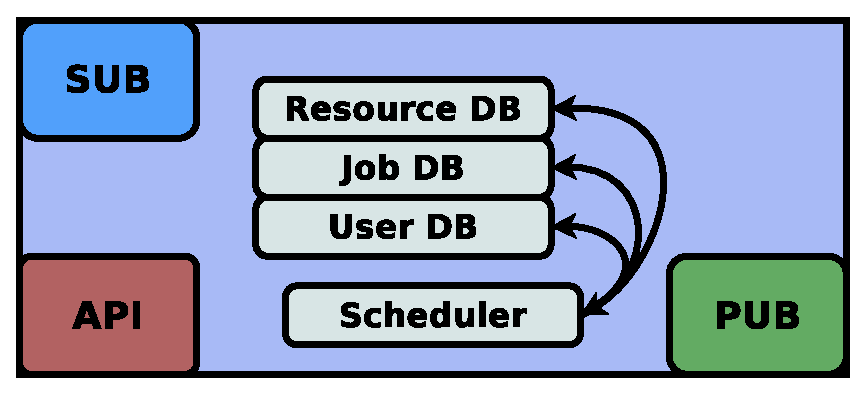
\includegraphics[scale=0.33]{RM-instance}
\end{center}
\end{slide}

% ==========================================================================
\overlays{8}{
\begin{slide}{\ngrm\ multi-instance instantiation}
\begin{center}
\onlySlide*{1}{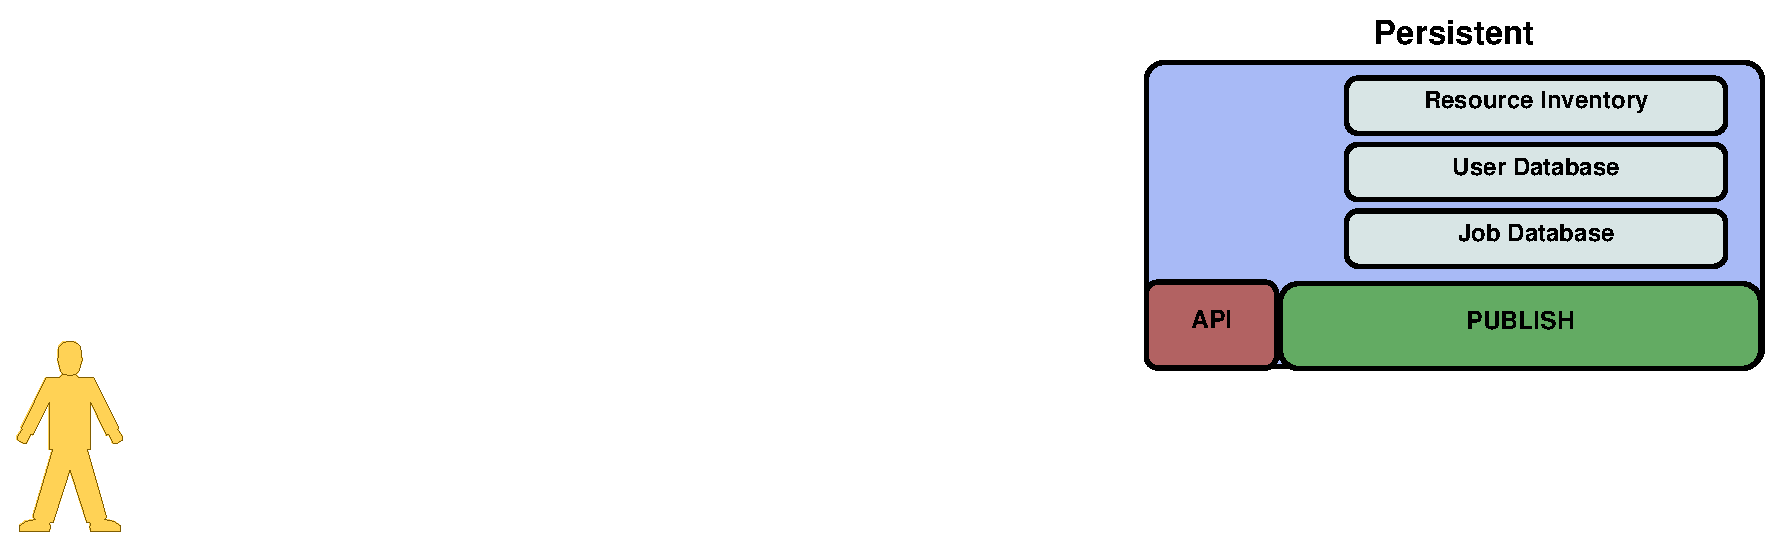
\includegraphics[scale=.2]{graphic/rm1}}
\onlySlide*{2}{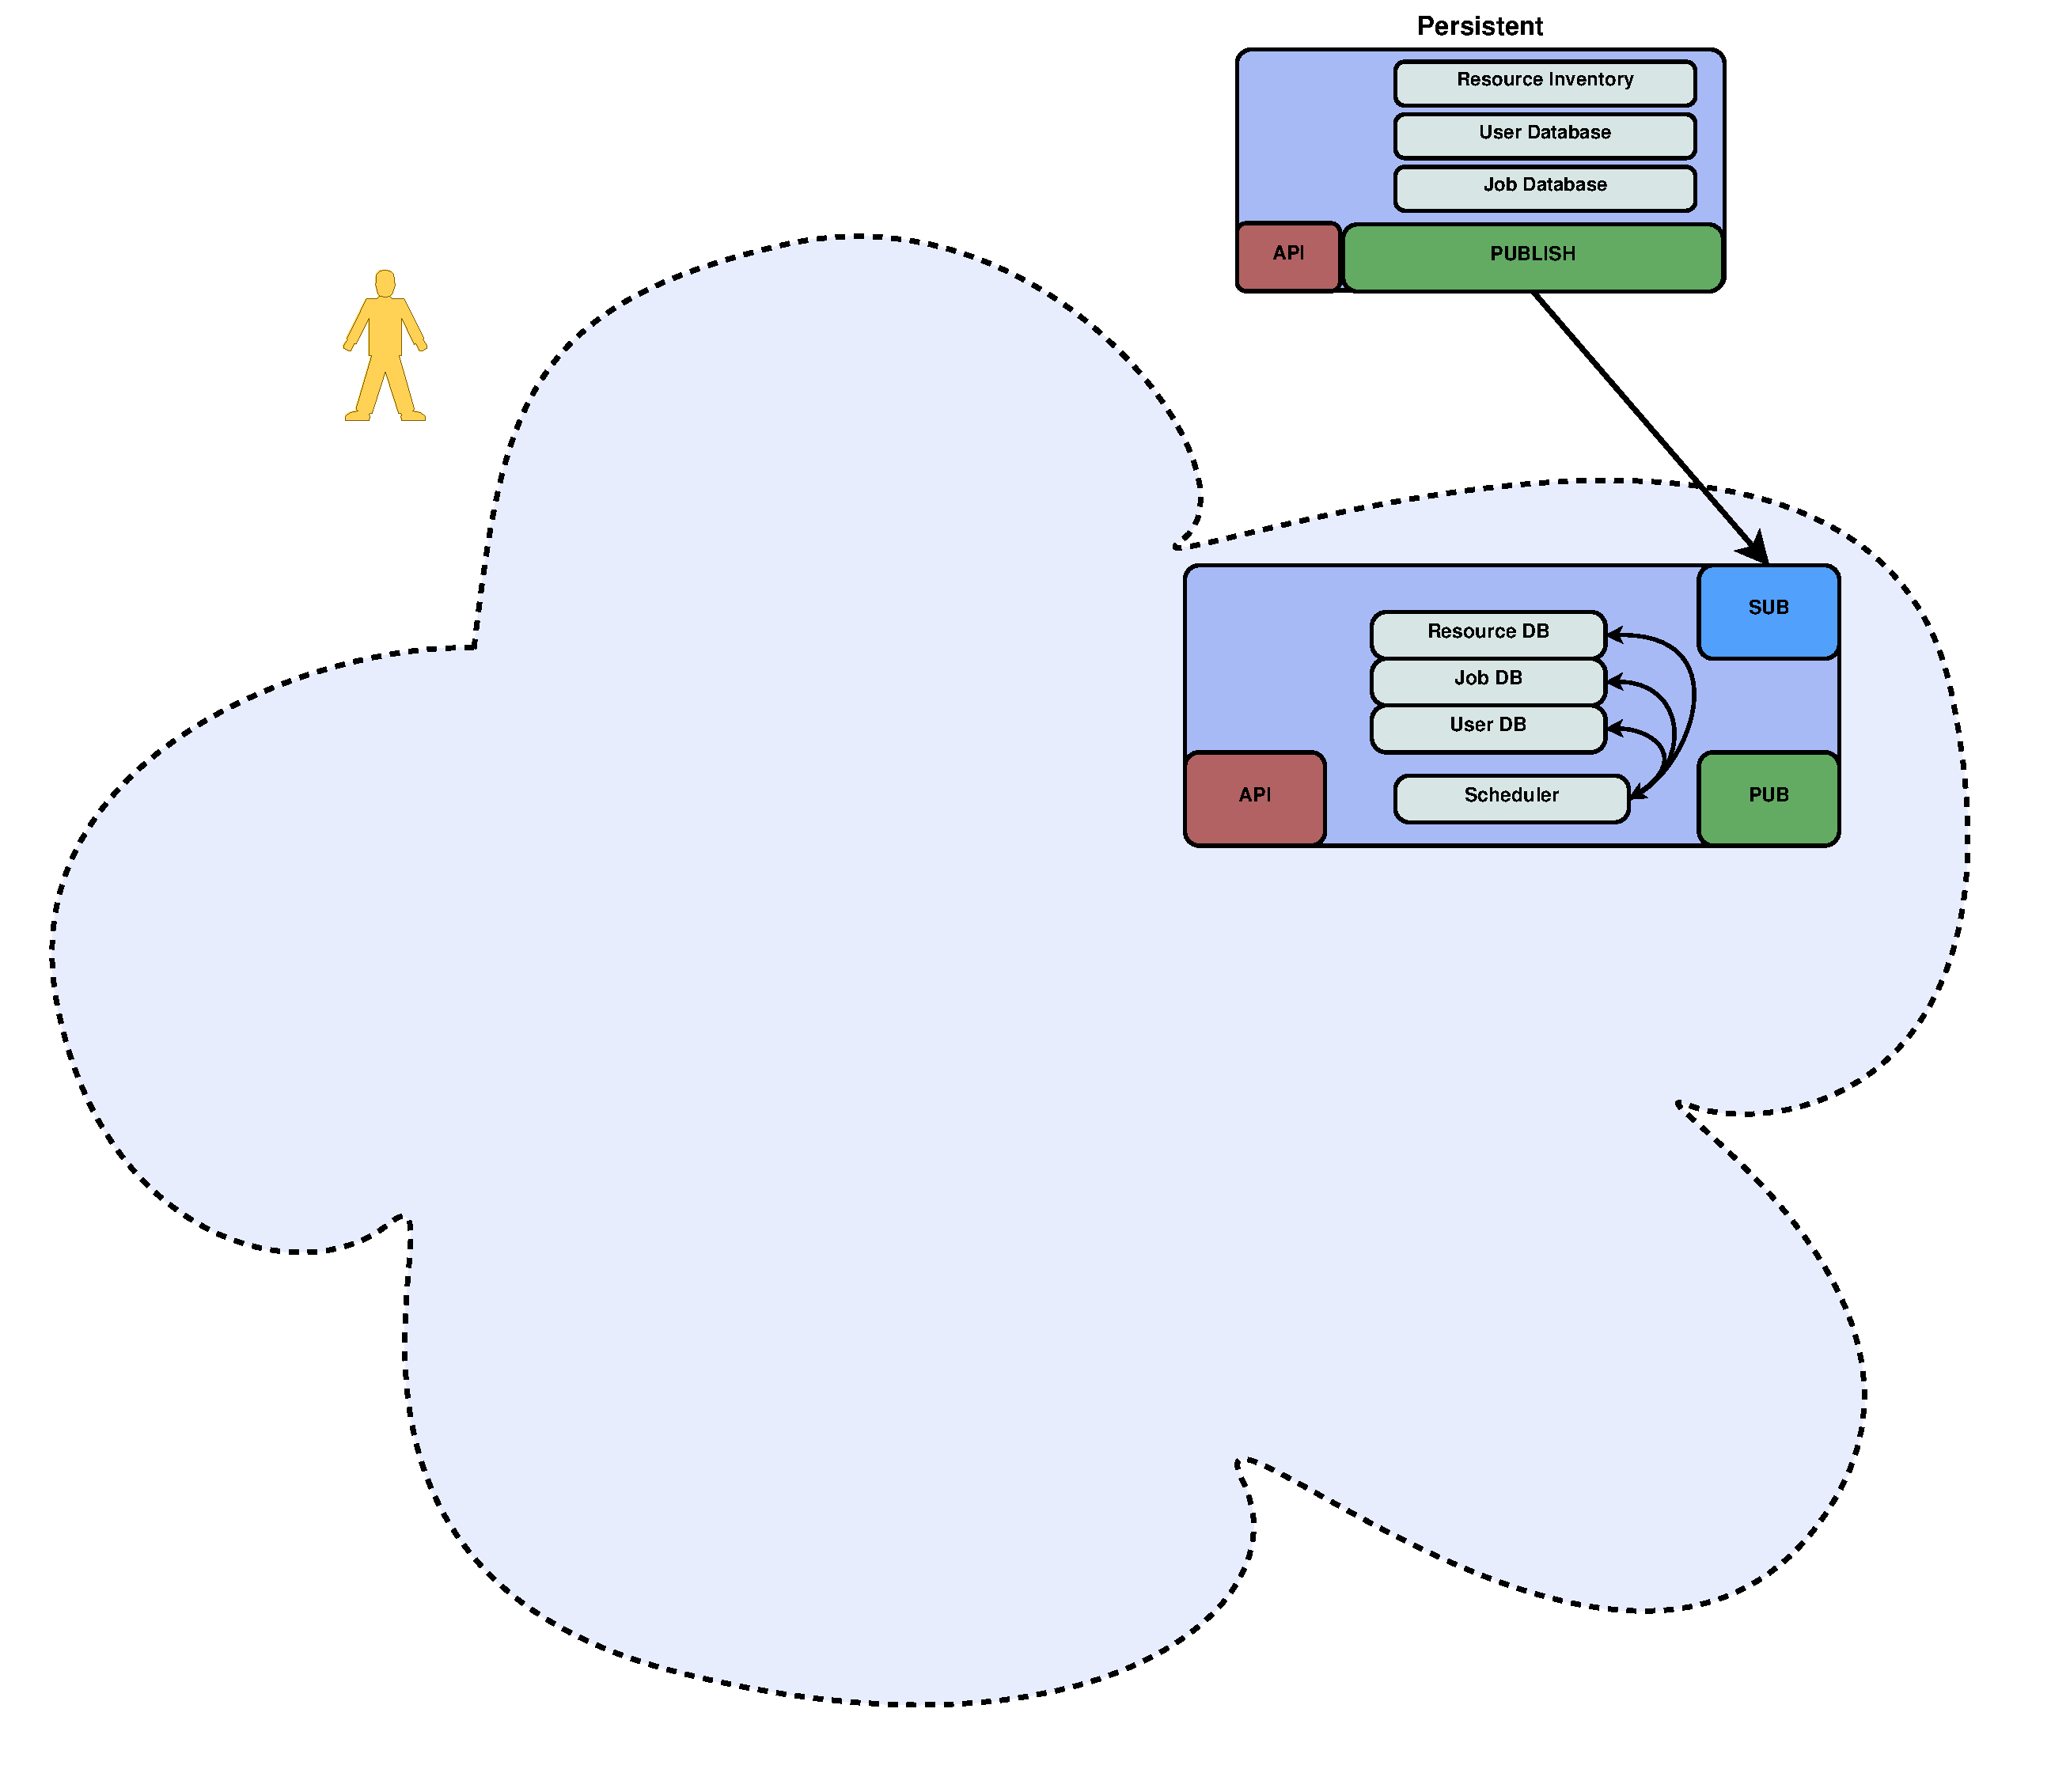
\includegraphics[scale=.2]{graphic/rm2}}
\onlySlide*{3}{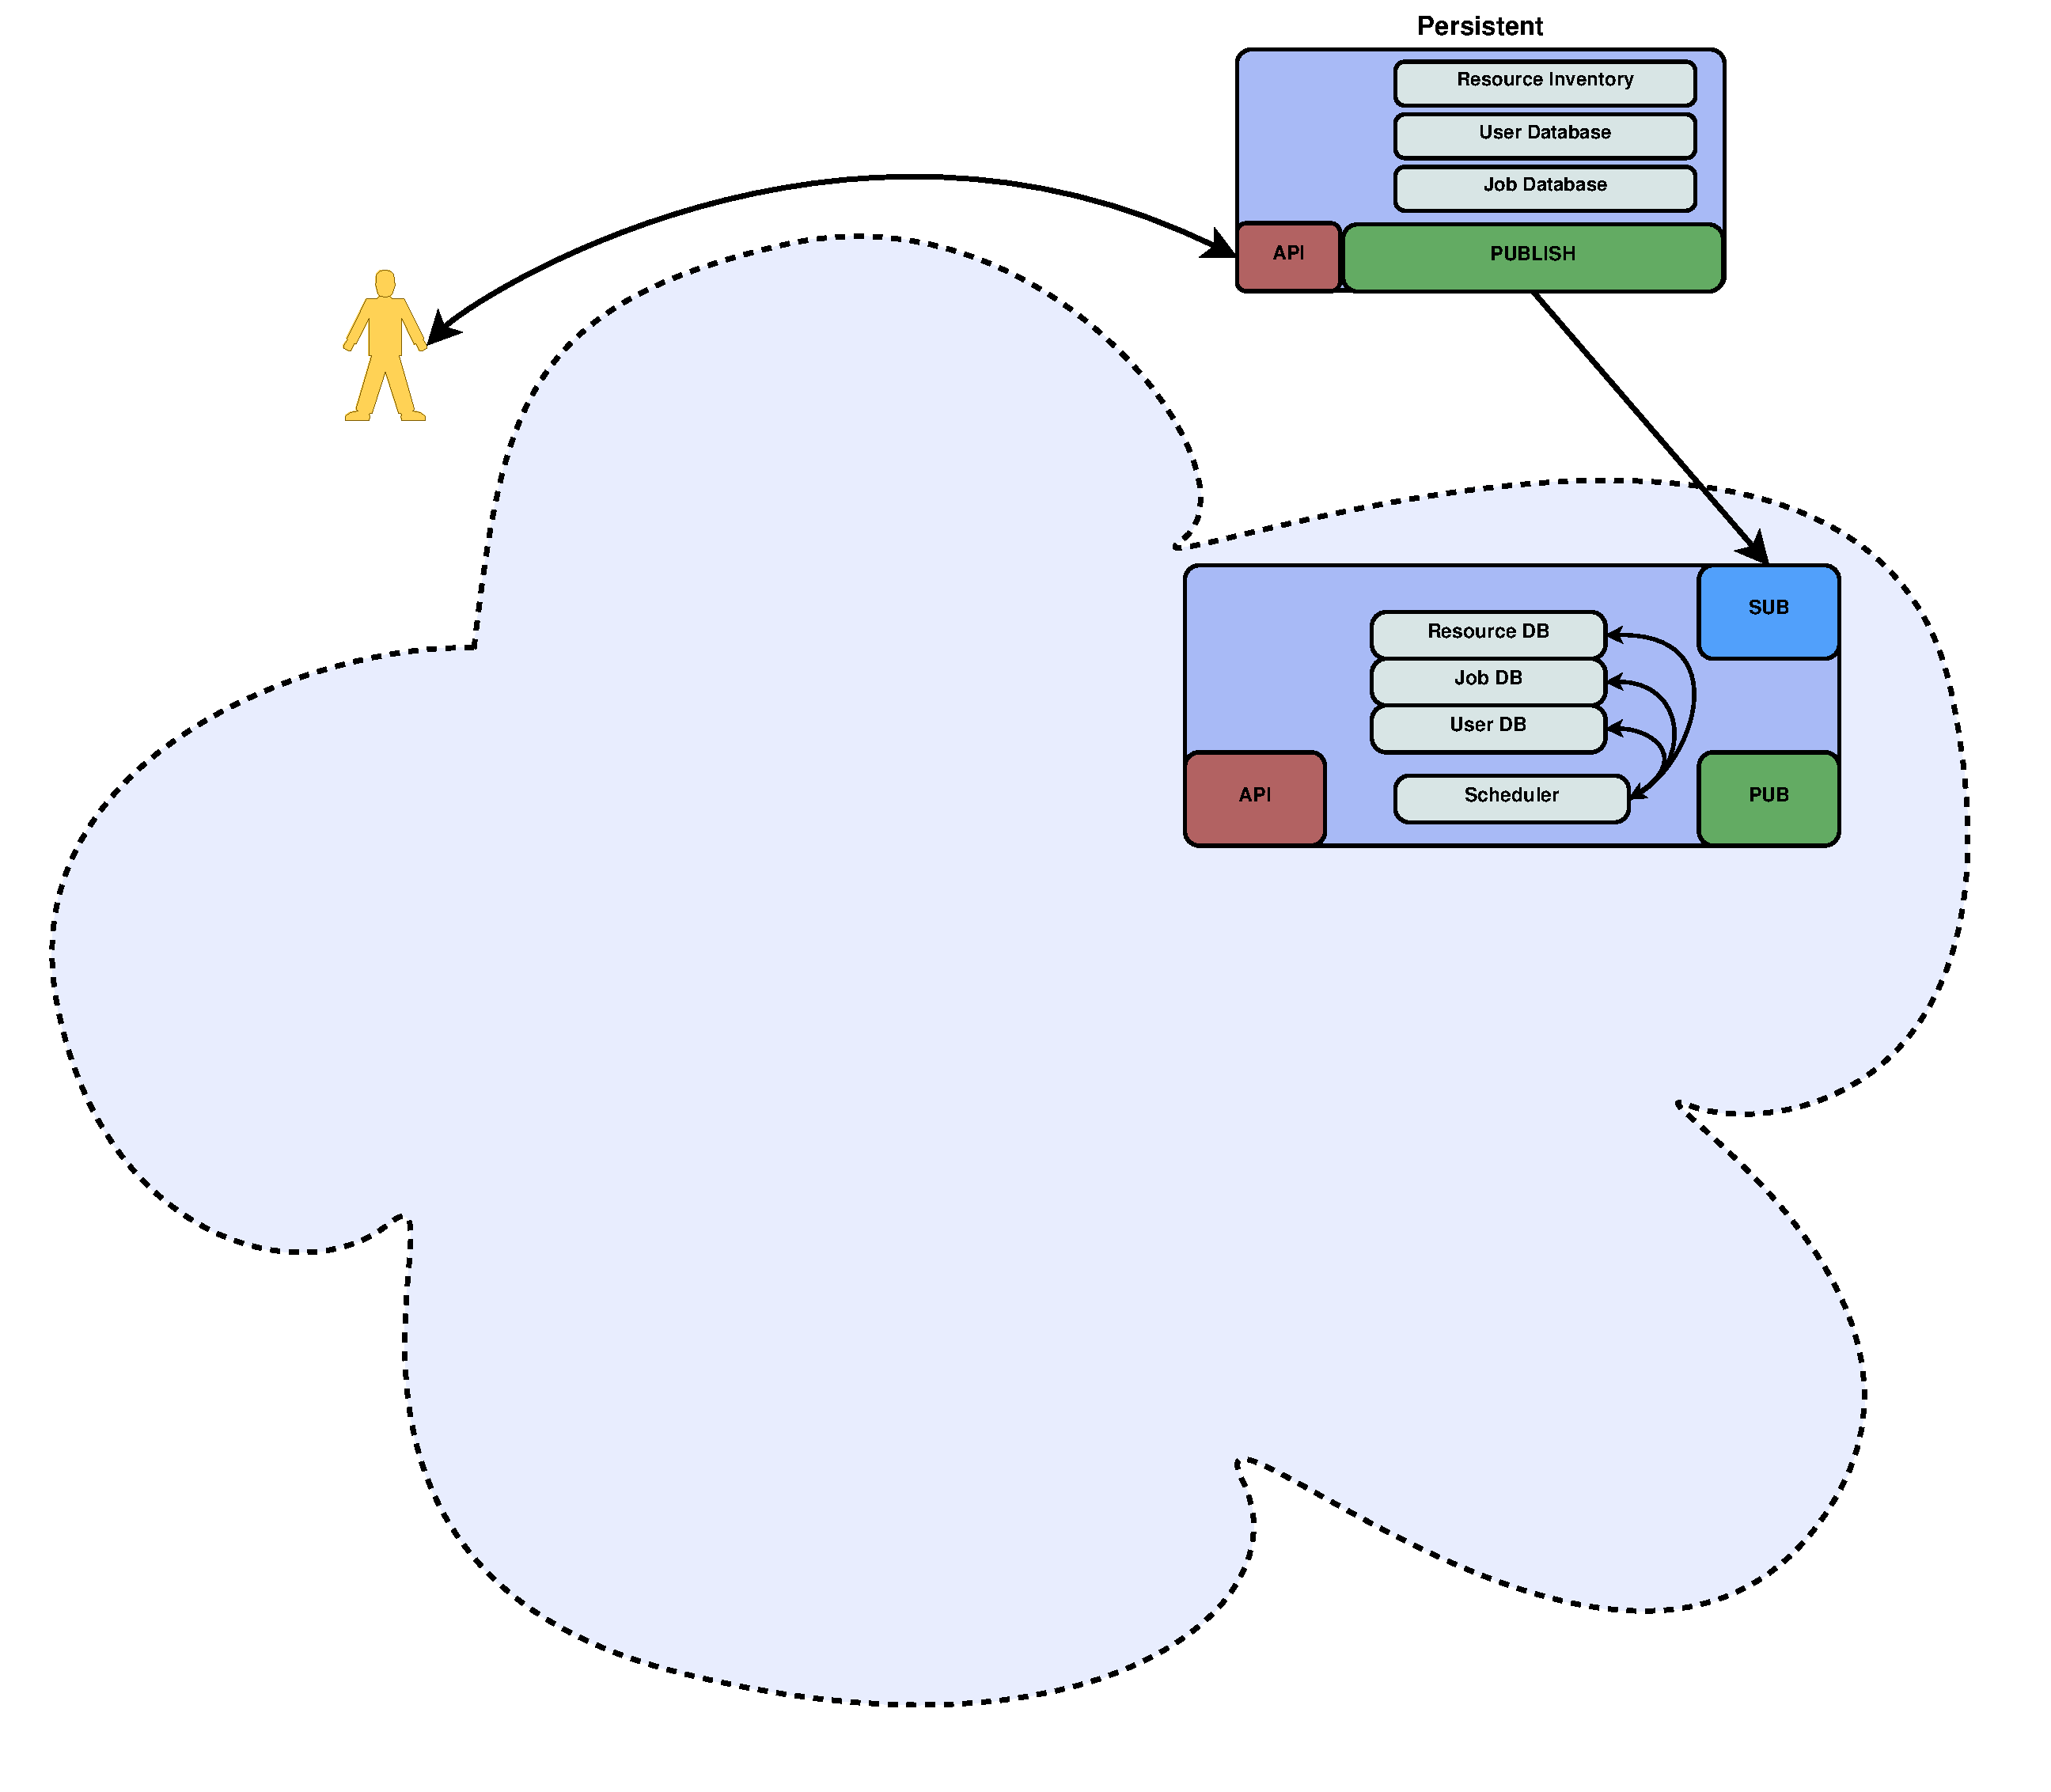
\includegraphics[scale=.2]{graphic/rm3}}
\onlySlide*{4}{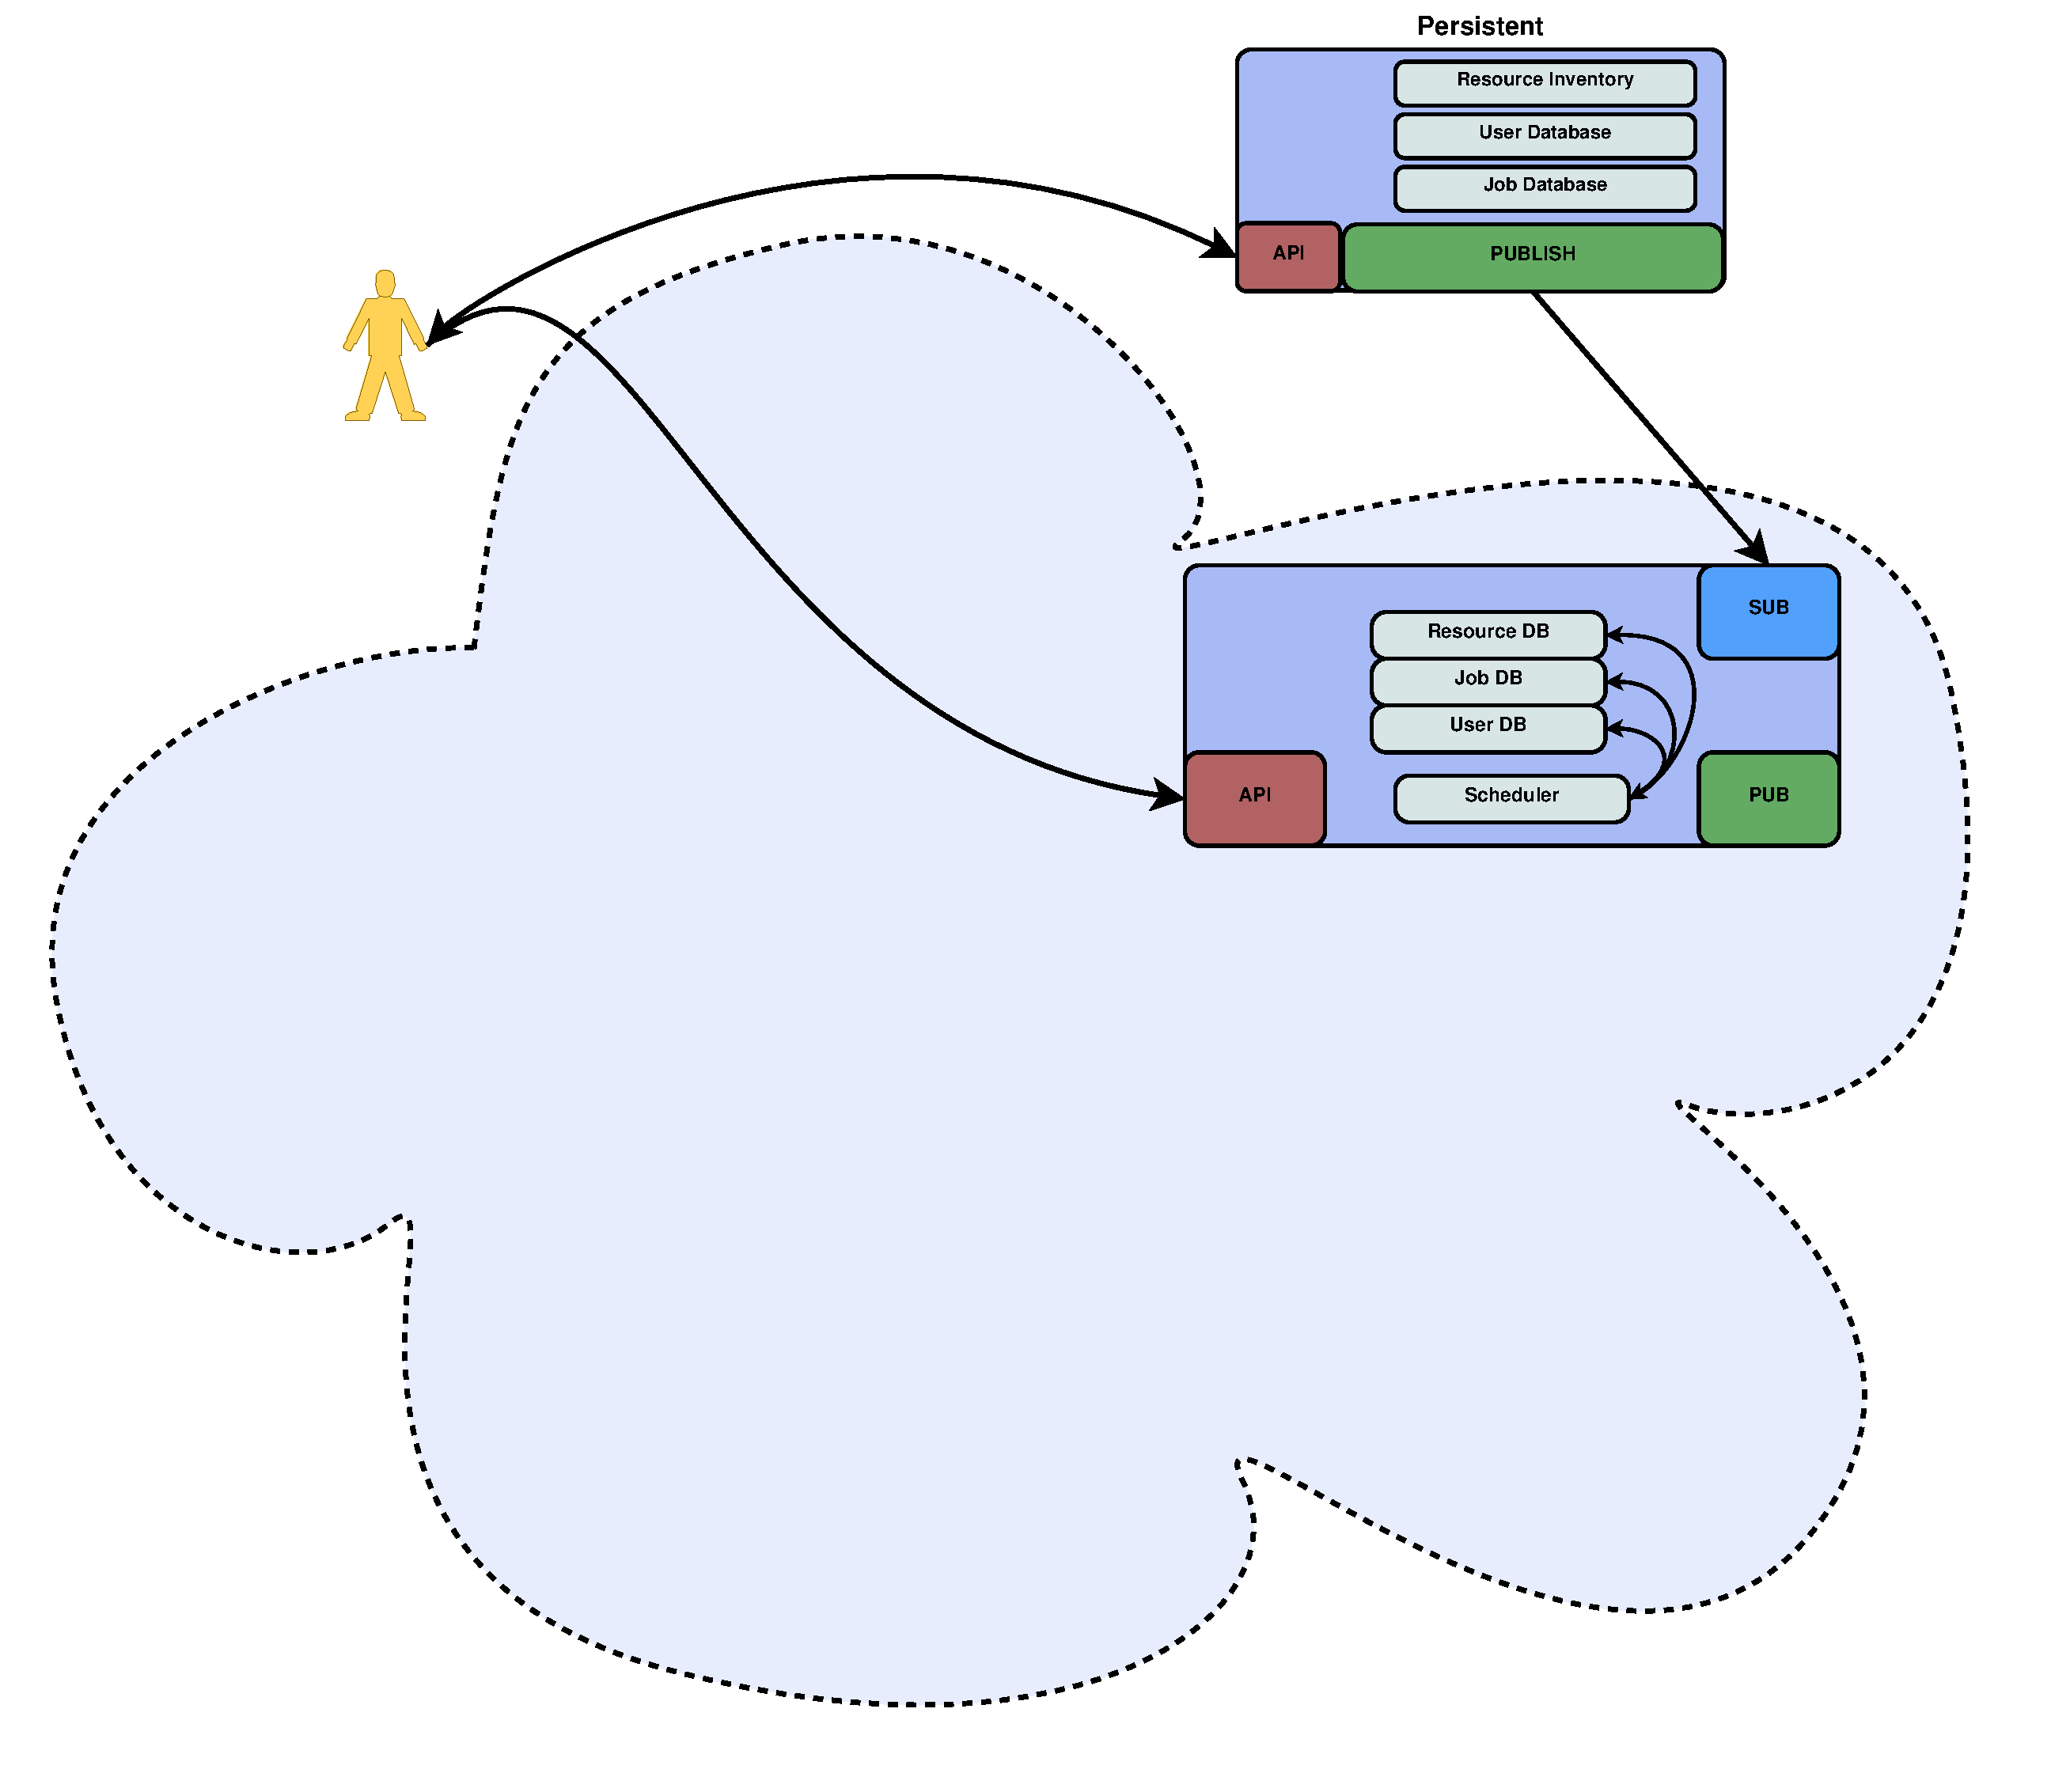
\includegraphics[scale=.2]{graphic/rm4}}
\onlySlide*{5}{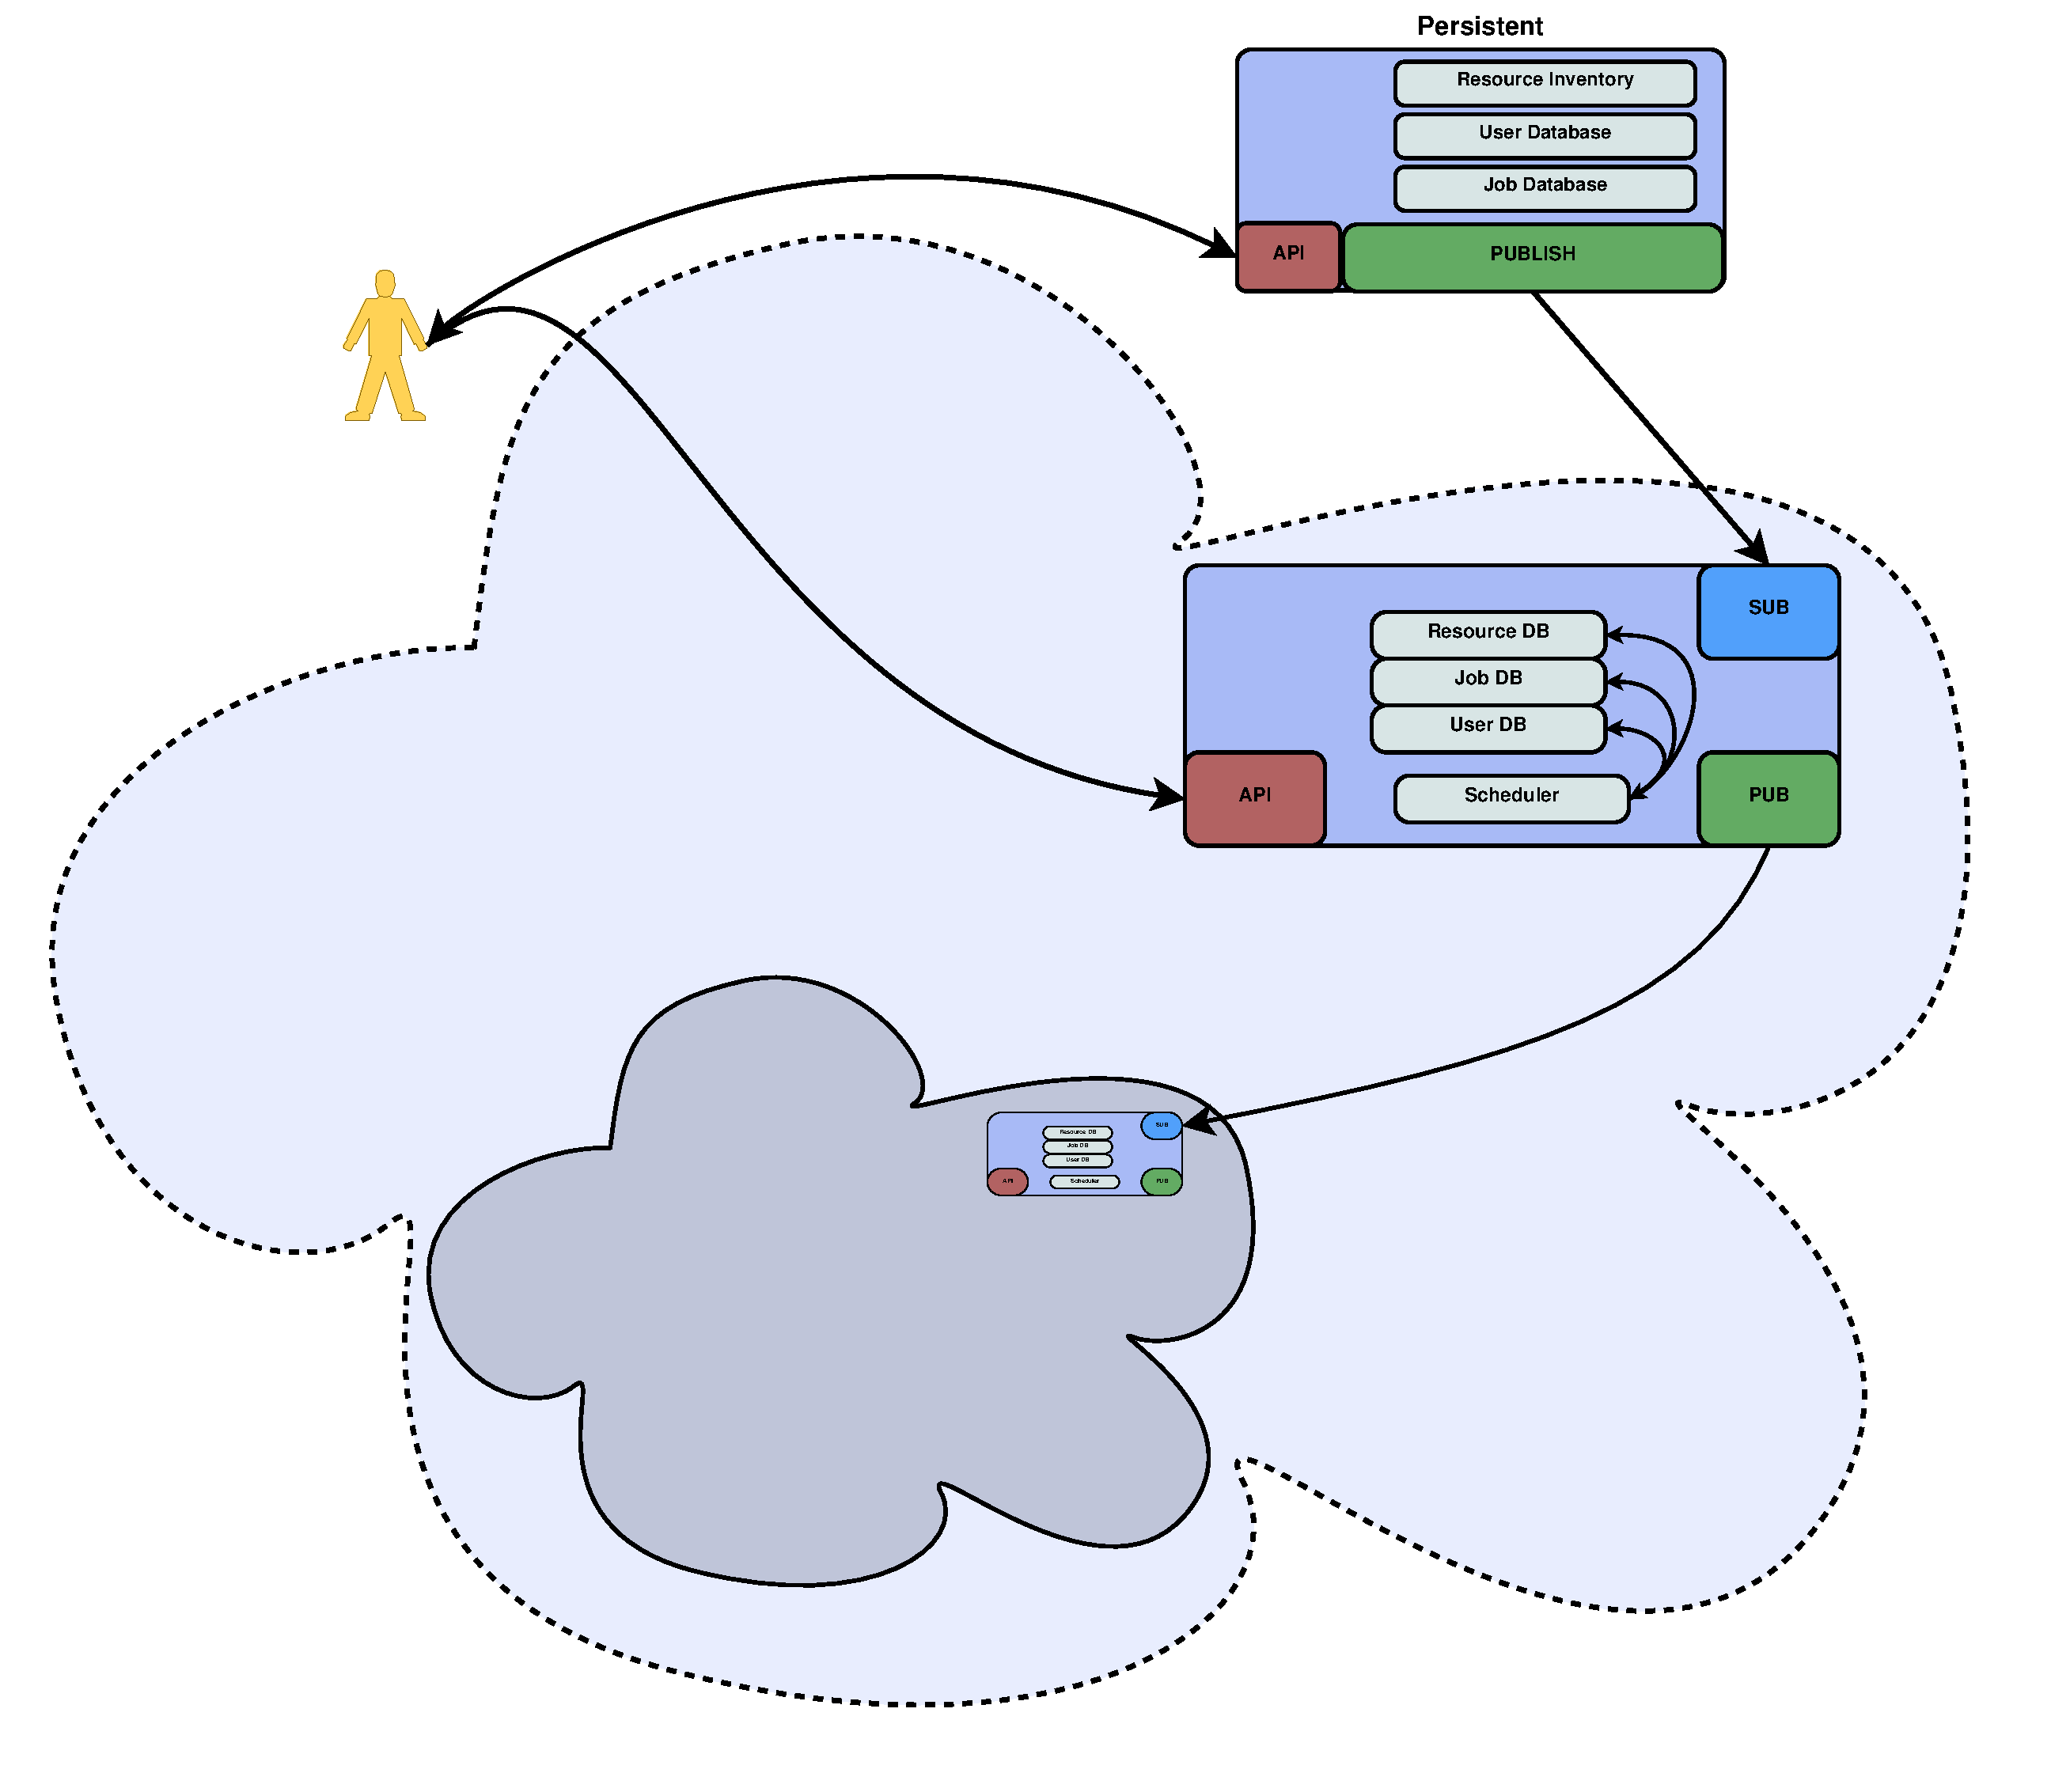
\includegraphics[scale=.2]{graphic/rm5}}
\onlySlide*{6}{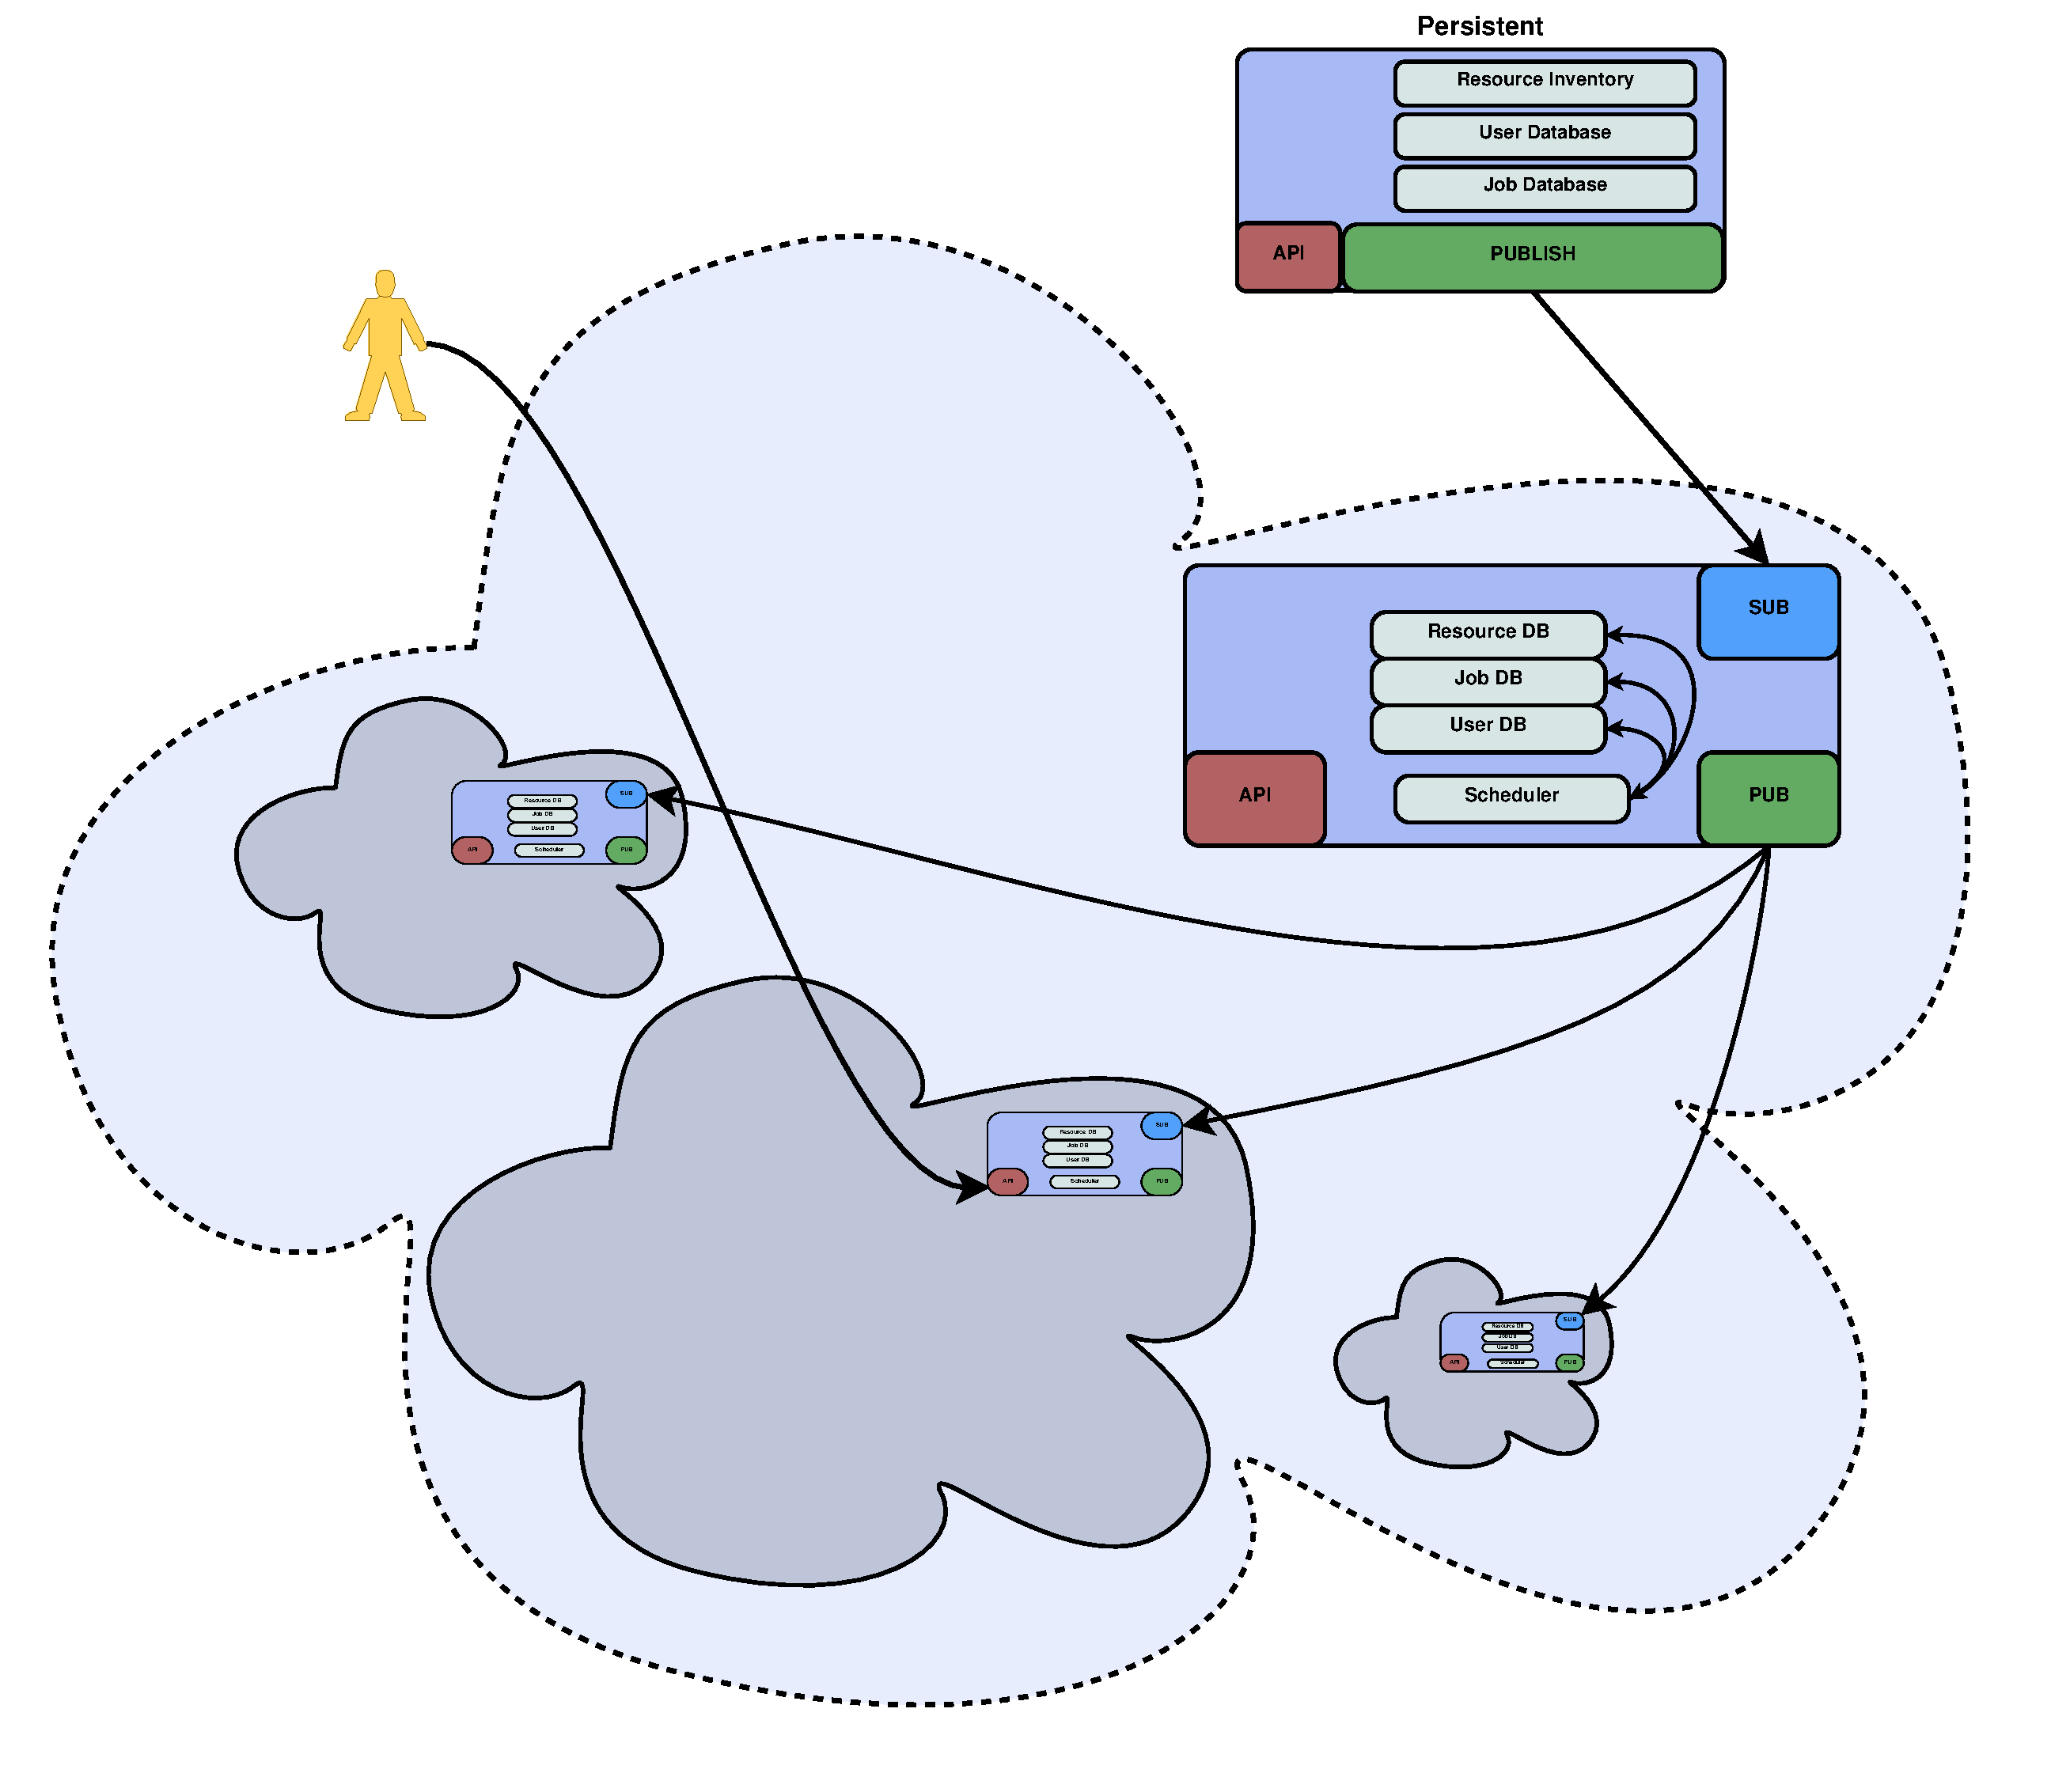
\includegraphics[scale=.2]{graphic/rm6}}
\onlySlide*{7}{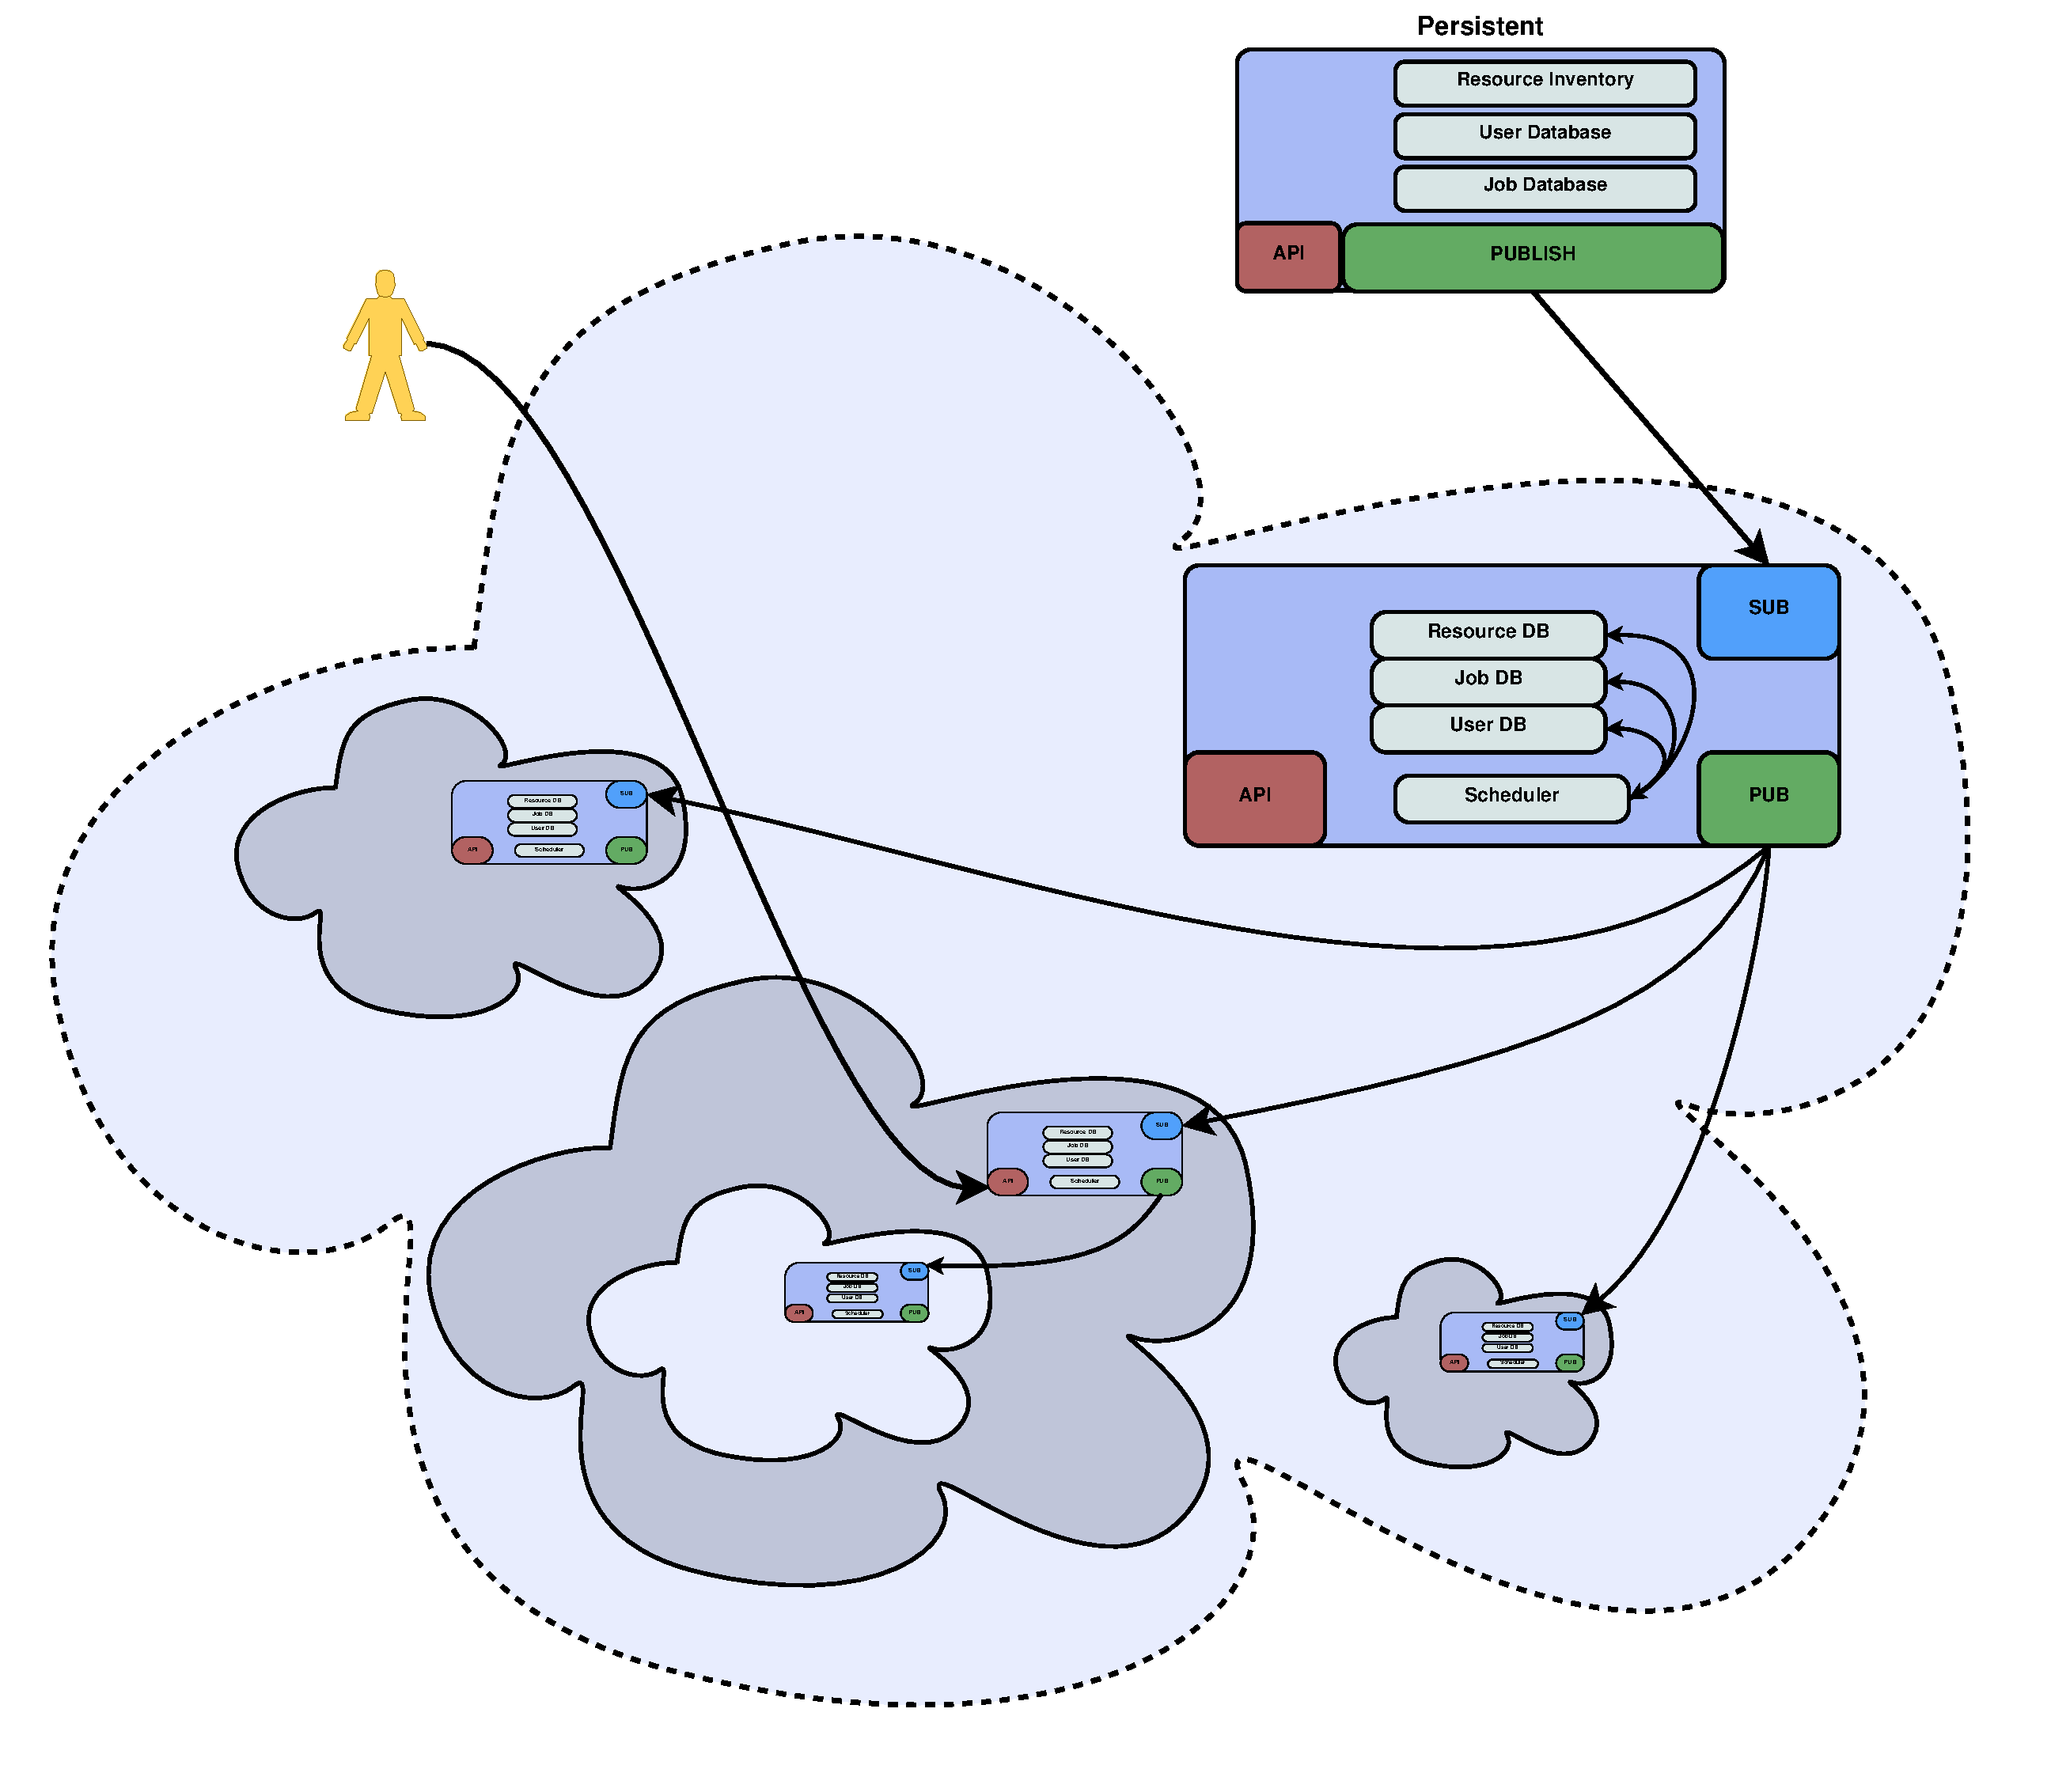
\includegraphics[scale=.2]{graphic/rm7}}
\onlySlide*{8}{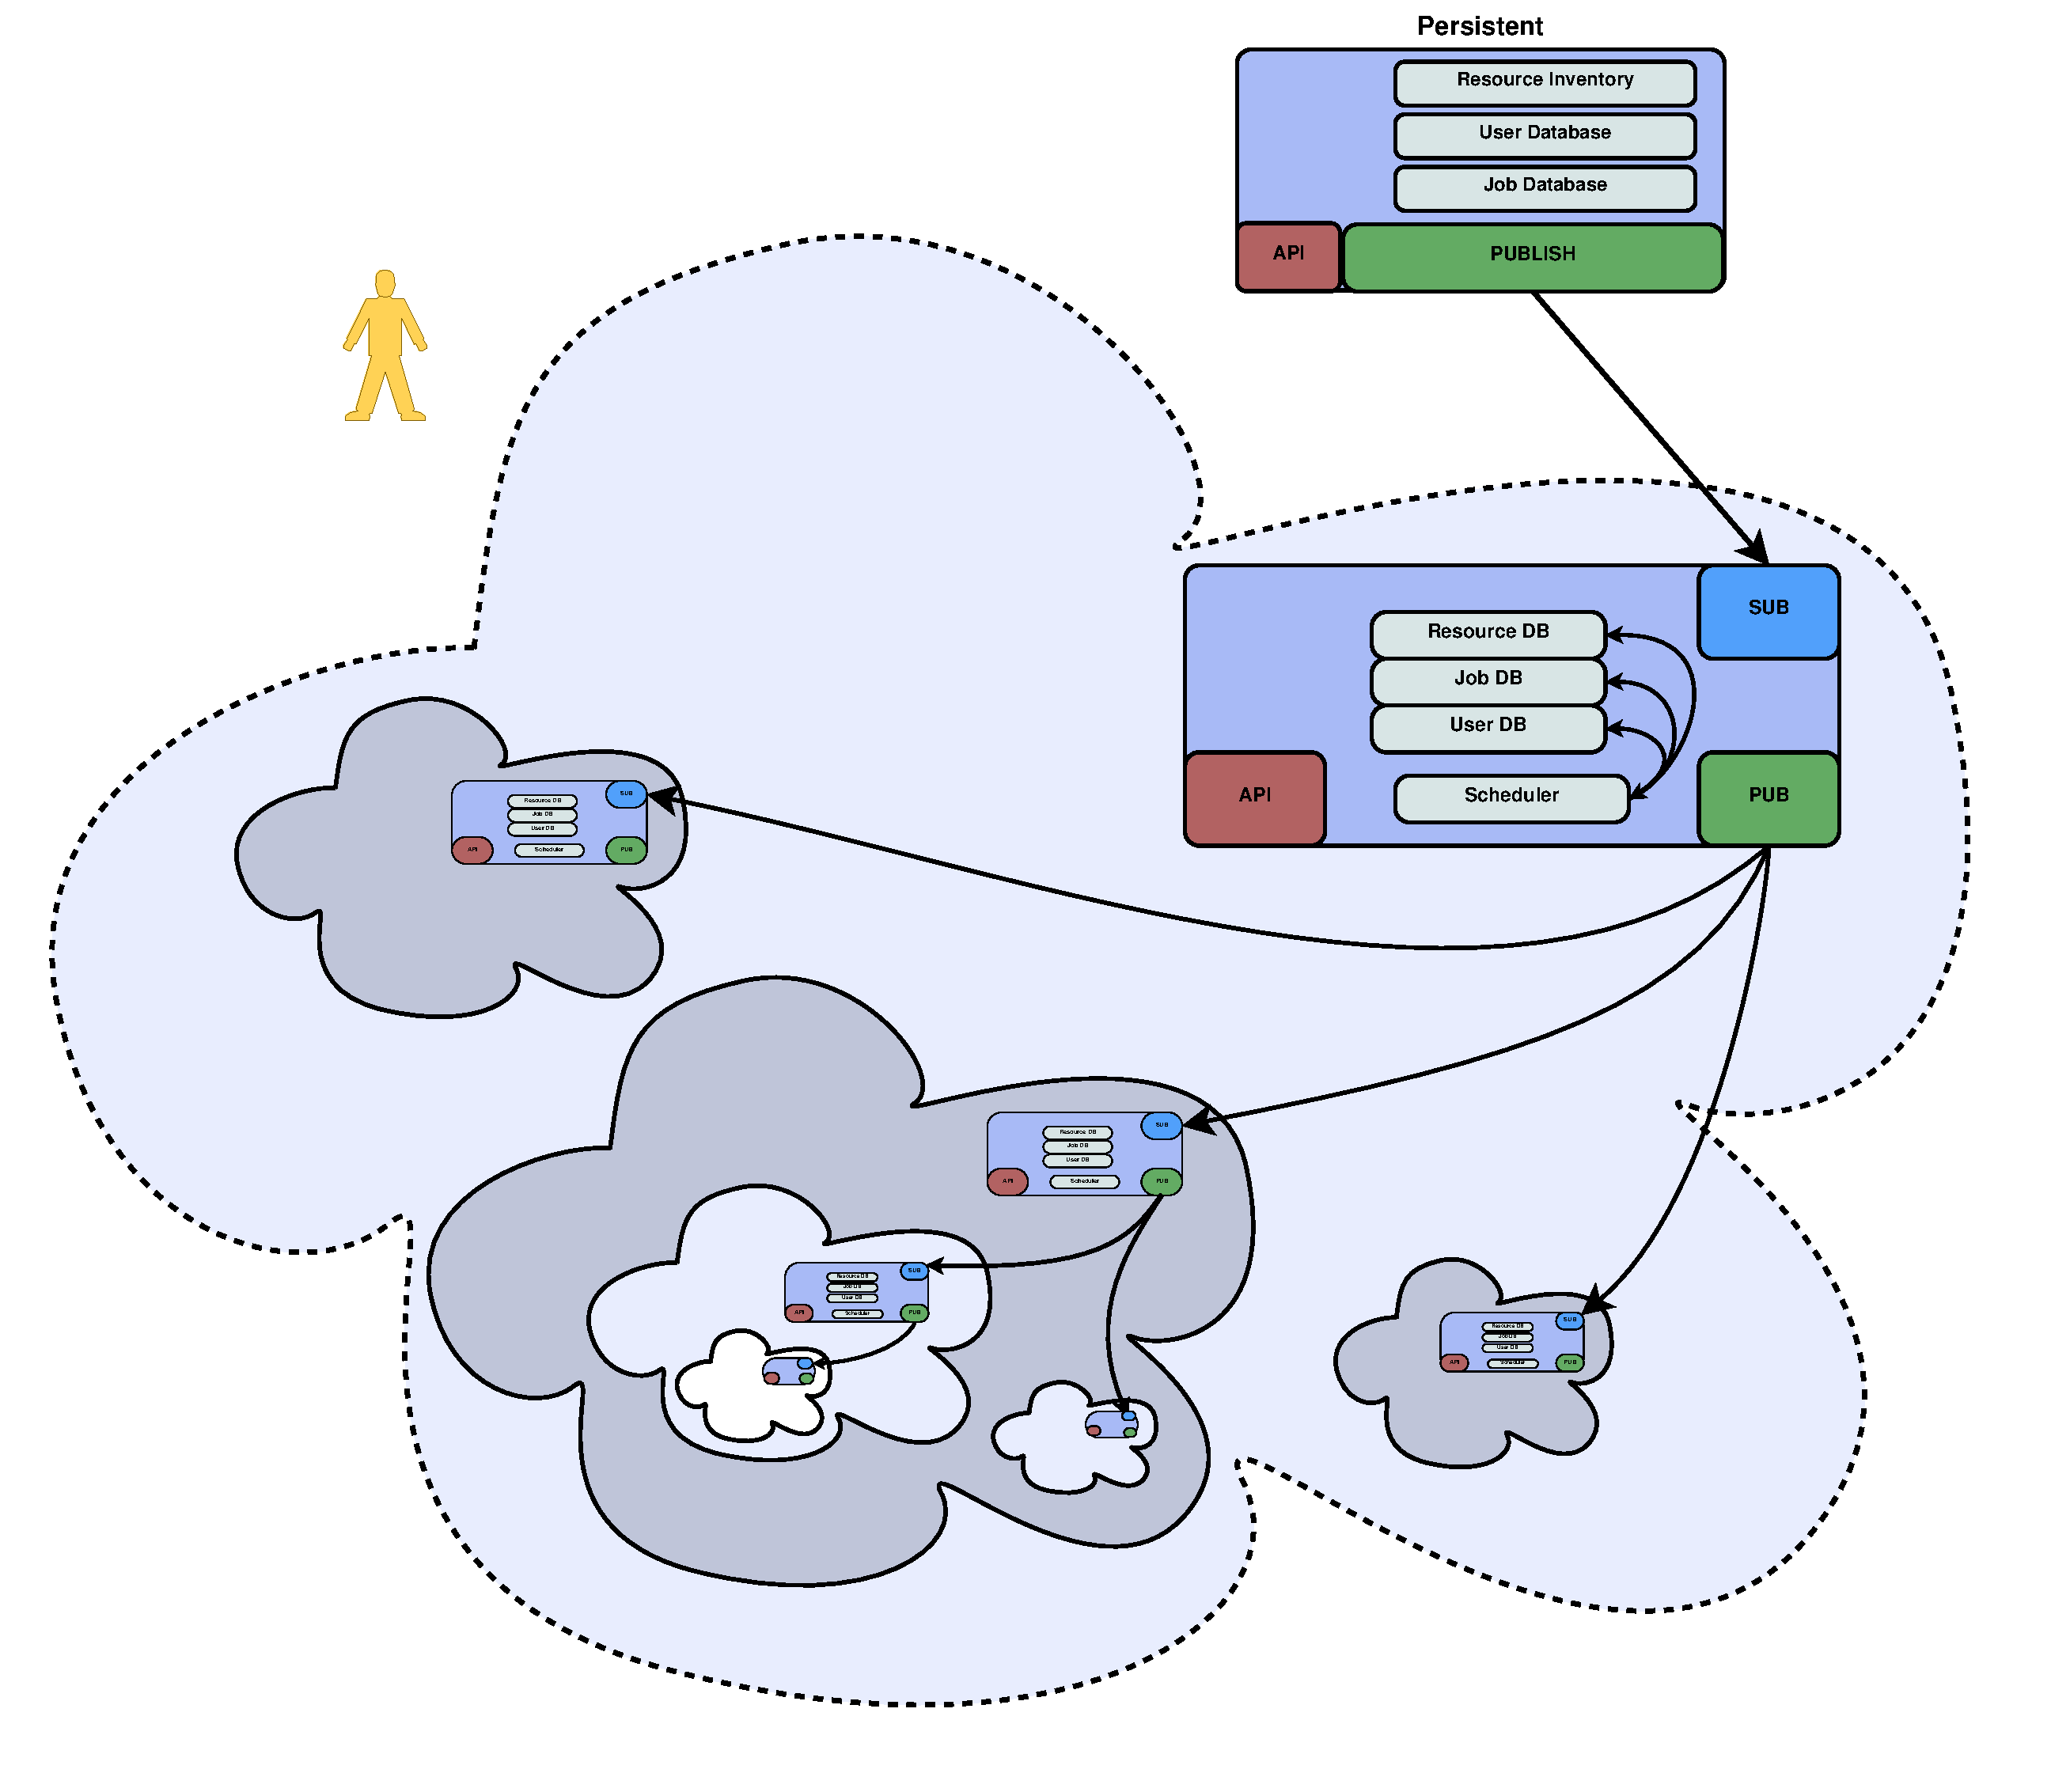
\includegraphics[scale=.2]{graphic/rm8}}
\end{center}
\end{slide}
}

% ==========================================================================
\end{document}
